	\marginpar{26.10.2015} Okay, Leute. Herr Prof. Bali hat heute eine Seite Korrektur an die Tafel geschrieben, aber ich weiß nicht wo jetzt welche 2 weg oder hin muss, denn am Ende wusste er es selbst auch nicht mehr. Deshalb schreibe ich einfach das auf, was ich mitgeschreiben habe. 

	Korrektur ! 
		\begin{align*}
			\vec{A} (\vec{r} , t) &=
			2 \mathrm{Re} \left(
				A_0 \vec{\epsilon} e^{i (\vec{k} \vec{r} - \omega t)}
			\right) \\
			|\vec{S}| &=
			c |\vec{E}| = \frac{\omega^2}{c} 4 |A_0|^2 \\
			u &= \frac{1}{2} \overline{\left( \vec{E}^2 + \vec{B}^2 \right)} 
			= \frac{1}{c} \overline{|\vec{S}|} 
			= \frac{\omega^2}{c^2} 2 |A_0|^2 = \frac{I}{c} \\
			H^1 &= \frac{e}{mc} \left[
				A_0 e^{i (\vec{k} \vec{r} - \omega t)} \vec{\epsilon} \vec{p} 
				+ A_0^\dagger e^{-i (\vec{k} \vec{r} - \omega t)} \vec{\epsilon} \vec{p}
			\right] \\
			&+ \frac{e^2}{m c^2} 4 |A_0|^2 \left( 1 + \cos (2 (\vec{k} \vec{r} - \omega t))\right) \\
			| \braket{m | H_\omega | n} |^2 &=	
			\frac{e^2}{4\!\!\!/ m^2 c^2} |A_0|^2
			| \braket{m | e^{i \vec{k} \vec{r}} \vec{\epsilon} \vec{p} | n} |^2 
			= \frac{e^2 u(\omega)}{2 m^2 \omega^2} 
			| \braket{m | e^{i \vec{k} \vec{r}} \vec{\epsilon} \vec{p} | n} |^2 \\
			W_{m \leftarrow n} &= \frac{4\!\!\!/ \pi e^2 u(\omega_{mn})}{m^2 \hbar^2 \omega_{mn}^2}
			|\braket{\ldots}|^2
		\end{align*}
		\begin{empheq}[box=\boxed]{align*}
			W_{m \leftarrow n} &=
			\frac{4 \pi^2 \alpha c}{\hbar^3 \omega_{mn}} u(\omega_{mn}) 
			| \braket{m | e^{i \vec{k} \vec{r}} \left[ H^0, \vec{r} \cdot \vec{\epsilon} \right]} |^2
		\end{empheq}
	Dipolnäherung:
		\begin{align*}
			W_{m \leftarrow n} &=
			\frac{4 \pi^2 \alpha c}{\hbar} u(\omega_{mn}) 
			| \braket{m | \vec{\epsilon} \cdot \vec{r} | n} |^2 
			= \frac{\pi}{\hbar^2} u(\omega_{mn}) 
			| \braket{m | \vec{\epsilon} \cdot \vec{d} | n} |^2
		\end{align*}
		\begin{align*}
			\int \diff \Omega_\epsilon \epsilon_i \epsilon_j &= c \delta_{ij} \\
			\text{Beispiel: ~} \epsilon_z &= \cos \Theta \\
			\int \diff \Omega_\epsilon \epsilon_z^2 &= 
			\int_{0}^{2 \pi} \diff \phi \int_{-1}^{1} \diff (\cos \Theta) \cos^2 \Theta 
			= 2 \pi \left. \frac{\cos^3 \Theta}{3} \right|_{-1}^1 = \frac{4 \pi}{3} \\
			\Rightarrow c &= \frac{4 \pi}{3} 
	 	\end{align*}
	 	\begin{empheq}[box=\boxed]{align*}
		 	W_{m \leftarrow n} = \frac{\pi}{3 \hbar^2} u(\omega_{mn})
		 	| \braket{n | \vec{d} | m} |^2
	 	\end{empheq}
	 	\begin{figure*} [h]
	 		\begin{center}
	 			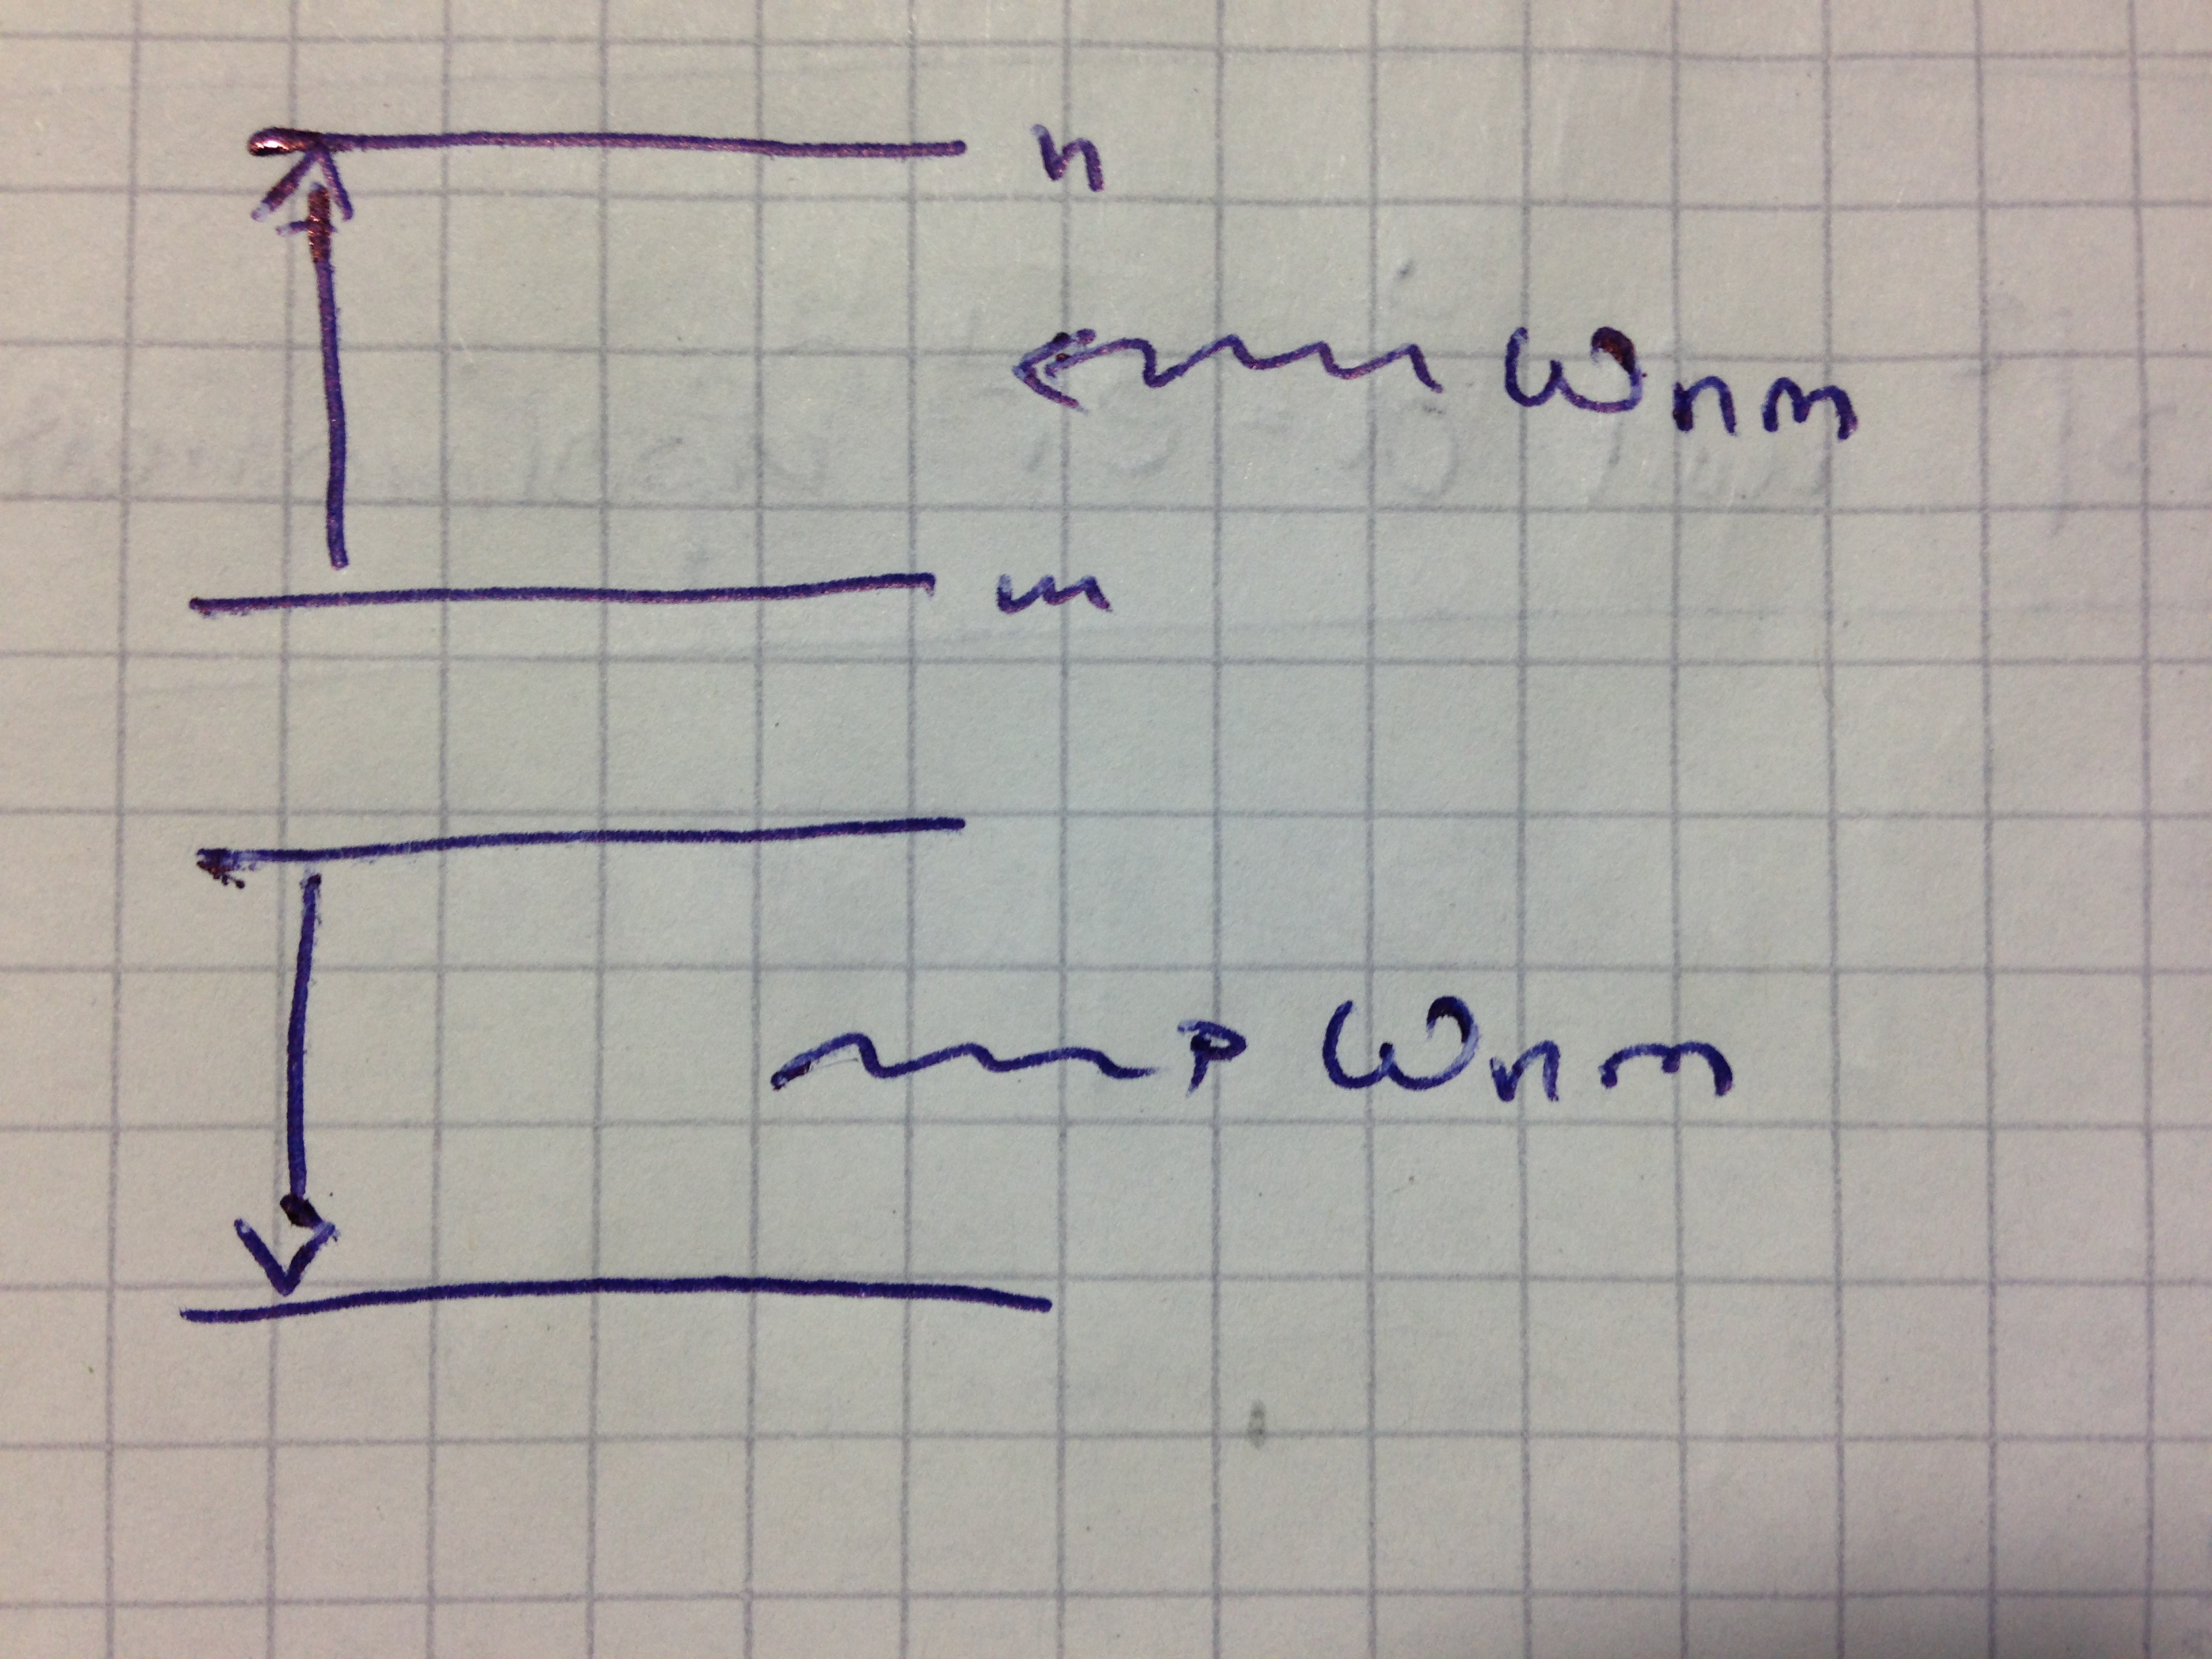
\includegraphics[width=10cm]{Bild1.jpg}
	 		\end{center}
		\end{figure*}
	\FloatBarrier
\subsection{Spontane Emissions}
	Ein genaues Verständnis dieses Phänomens erfordert eine Quantentheorie des elektromagnetischen Feldes, die man Quantenelektrodynamik (QED) nennt. 
	\\
		
	Betrachte Kasten des Volumens $V = L^3$ \\	
	(Nebenbemerkung: Bei $L \rightarrow \infty$ gibt es infratrot ``Probleme'')
		\begin{align*}
			\vec{A} (\vec{r} , t) &= \vec{\epsilon}~ e^{i (\vec{k} \vec{r} - \omega_k t)} 
			,& \omega_k &= |\vec{k}| \cdot c 
		\end{align*}
	2 orthogonale Polarisationsrichtungen: 
		\begin{align*}
			\vec{\epsilon}_+ \cdot \vec{\epsilon}_- &= 0 
			,& &\vec{k} \cdot \vec{\epsilon}_\pm = 0 \\
			& & &(\text{transversale Welle~} \vec{\nabla} \vec{A} = 0 )
 		\end{align*}
 		\begin{align*}
	 		\vec{\epsilon}_\lambda ~,~ \lambda &\in \{ - , + \} \\
	 		\vec{A} (\vec{r} + L \vec{e}_x , t) &= \vec{A} (\vec{r} , t) &
	 		&\text{für periodische (nicht wichtig) Randbedingungen.} \\
	 		\Rightarrow \vec{k} L \vec{e}_x &= k_x L = 2 \pi n_x &
	 		&\left( e^{i \vec{k} \vec{r}} = e^{i \vec{k} (\vec{r} + L \vec{e}_x)} \right) \\
	 		n_x &\in \mathds{Z}. \\
	 		\vec{k} &= \frac{2 \pi}{L} \vec{n} ,& &n_x, n_y, n_z \in \mathds{Z}
 		\end{align*}
 	Allgemeines
	 	\begin{align*}
		 	\vec{A} (\vec{r} , t) = \frac{c}{\sqrt{2 V}}
		 	\sum_{\vec{k}} \sum_{\lambda \in \{+ , - \} }
		 	\vec{\epsilon}_\lambda (\vec{k}) 
		 	\underbrace{q_\lambda}_{\mathclap{\in \mathds{C}}} (\vec{k} , t) 
		 	e^{-i \vec{k} \vec{r}}
	 	\end{align*}
	Wir fordern $\vec{A} \in \mathds{R}^3$.
		\begin{align*}
			\Rightarrow q_\lambda (- \vec{k} , t) &= q^*_\lambda (\vec{k} , t) ,&
			&\vec{\epsilon}_\lambda (-\vec{k}) = \vec{\epsilon}_\lambda (\vec{k}) \\
			\text{Zusätzlich:~} q_\lambda (\vec{0} , t) &= 0 .& 
			&\text{(nur ebene Wellen)}
		\end{align*}
	Wellengleichung: 
		\begin{align*}
			\left(
				\vec{\nabla}^2 - \frac{1}{c^2} \frac{\partial^2}{\partial t^2} 
			\right)
			\vec{A} (\vec{r} , t) &= \overbrace{0}^{\mathclap{\text{im Vakuum}}} \\
			\overset{\text{Koeff.-Vergleich}}{\Rightarrow} 
			\frac{1}{c^2} \ddot{q}_\lambda (\vec{k} , t) + \vec{k}^2 q_\lambda &= 0
		\end{align*}
		\begin{align*}
			\boxed{\ddot{q}_\lambda (\vec{k} , t) + \omega_k^2 ~q_\lambda (\vec{k} , t)} = 0
		\end{align*}
	$q_\lambda$: Lösungen des harmonischen Oszillators mit Frequenz $\omega_k$. \\
	Energie des elektromagnetischen Feldes: 
		\begin{align*}
			E &= \int_V \diff^3 r ~u (\vec{r} , t) \\
			&= \int_V \diff^3 r \frac{1}{2} \left( \vec{E}^2 (\vec{r} , t) \vec{B}^2 (\vec{r} , t)
			\right) \\
			&= \frac{1}{2} \int_V \diff^3 r \left[
				\left(\frac{1}{c^2} \frac{\partial \vec{A}}{\partial t}\right)^2
				+ \left( \vec{\nabla} \times \vec{A}\right)^2
			\right] \\
			\left( \vec{\nabla} \times \vec{A}\right)^2 &=
			\vec{\nabla} \left(\vec{A} \times \left( \vec{\nabla} \times \vec{A} \right)\right)
			+ \left(\vec{A} \cdot \vec{\nabla}\right) 
			\underbrace{\left( \vec{\nabla} \cdot \vec{A}\right)}_{\mathclap{=0 \text{~(Coulombeichung)}}}
			- \vec{A} \cdot \vec{\nabla}^2 \cdot \vec{A} \\
			\text{zu der Klammer~} &\text{mit mehreren Rotationen:~} \\
			\int_V \diff^3 r~ \vec{\nabla} (\ldots) 
			&= \int_{\partial V} \diff^2 r~ \vec{n} (\vec{r}) (\ldots) = 0
		\end{align*}
		\begin{align*}
			\boxed{
				E = \frac{1}{2} \int \diff^3 r \left[ 
				\left(\frac{1}{c} \frac{\partial \vec{A}}{\partial t}\right)^2
				- \vec{A}~ \vec{\nabla}^2 \vec{A}
				\right]	
			}
		\end{align*}
	Nebenrechnung:
		\begin{align*}
			\int \diff^3 r (\dot{\vec{A}})^2 &= 
			\frac{c^2}{2 V} \sum_{\vec{k}, \lambda} \sum_{\vec{k}', \lambda'}
			\underbrace{\int \diff^3 r e^{i (\vec{k} + \vec{k}') \vec{r}}}_{
				\substack{V \delta_{\vec{k}, -\vec{k}} 
					\text{~für diskretes~} \vec{k},\\ 
					(2 \pi)^3 \delta^{(3)} (\vec{k} + \vec{k}') \\ 
					\text{~kontinuierliches~} \vec{k}}
				}
			\vec{\epsilon}_\lambda(\vec{k}) ~\vec{\epsilon}_{\lambda'} (\vec{k}')
			~\dot{q}_\lambda (\vec{k} , t) ~\dot{q}_{\lambda'} (\vec{k}' , t) 
			\\
			&\overset{\vec{k}' = -\vec{k}'}{=} 
			\frac{c^2}{2} \sum_{\vec{k}, \lambda, \lambda'}
			\vec{\epsilon}_\lambda (\vec{k}) ~\vec{\epsilon}_{\lambda'}(-\vec{k})~
			\dot{q}_\lambda (\vec{k} , t) ~\dot{q}_{\lambda'} (\vec{-k} , t)
			\\
			&= \frac{c^2}{2} \sum_{\vec{k}, \lambda, \lambda'}
			\vec{\epsilon}_\lambda (\vec{k}) ~\vec{\epsilon}_{\lambda'}(-\vec{k})~
			\dot{q}_\lambda (\vec{k} , t) ~\dot{q}^*_{\lambda'} (\vec{k} , t)
			\\
			&= \frac{c^2}{2} \sum_{\vec{k}} \sum_{\lambda \in \{+ , - \} }
			| \dot{q}_\lambda(\vec{k} , t)  |^2
		\end{align*}
	Analog:
		\begin{align*}
			\int_V \diff^3 r \left(- \vec{A} \vec{\nabla}^2 \vec{A}\right)
			&\overset{\text{part. Int.}}{=} \int_V \diff^3 r \left( \vec{\nabla} \vec{A} \right)^2 \\
			&= \frac{c^2}{2} \sum_{\vec{k}} \sum_{\lambda \in \{+ , - \} }
			\vec{k}^2 |q_\lambda (\vec{k} , t)|^2 \\
			E &= \frac{1}{4} \sum_{\vec{k} , \lambda} \left[
				|\dot{q}_\lambda (\vec{k} , t)|^2 + \omega^2_k |q_\lambda (\vec{k} , t)|^2
			\right] \\
			\text{wobei~} |\dot{q}_\lambda (\vec{k} , t)|^2 &= 
			\dot{q}_{1 \lambda}^2 (\vec{k} , t) + \dot{q}_{2 \lambda}^2 (\vec{k} , t) 
			\\
			\text{und~} 
			q_\lambda (\vec{k} , t) &= q_{1 \lambda} (\vec{k} , t) + i q_{2 \lambda} (\vec{k} , t) 
			,& q_{i \lambda} (\vec{k} , t) &\in \mathds{R} 
			\\
			q_\lambda (-\vec{k} , t) &= q_\lambda^* (\vec{k} , t) 
			&\Rightarrow q_{1 \lambda} (-\vec{k} , t) &= q_{1 \lambda} (\vec{k} , t) 
			\\
			& & q_{2 \lambda} (-\vec{k} , t) &= - q_{2 \lambda} (\vec{k} , t)			
		\end{align*}
		\begin{align*}
			E = \frac{1}{2} \sum_{\vec{k} \in H, \lambda}
			\left[
				\dot{q}_{1 \lambda}^2 (\vec{k} , t)
				+ \omega_k^2 ~q_{1 \lambda}^2 (\vec{k} , t)
				+ \dot{q}_{2 \lambda}^2 (\vec{k} , t)
				+ \omega_k^2 ~q_{2 \lambda}^2 (\vec{k} , t)
			\right]
		\end{align*}
	$\vec{k} \in H$ bedeutet $\vec{k}$ ist im Halbraum. z.B. $k_z > 0$
		\begin{align*}
			\text{für~} k_z &= 0 : k_y > 0 \\
			\text{für~} k_z &= k_y = 0 : k_x > 0 
		\end{align*}
	Zu jedem Wellenvektor $\vec{k} \in$ Halbraum und Polarisation $\lambda$ gehören je 2 harmonische Oszillatoren.	
		\begin{align*}
			H_{\text{harm.Oszil.}} &= 
			\frac{p^2}{2 m} + \frac{1}{2} m \omega^2 q^2 \\
			&= \frac{p^2}{2} + \frac{\omega^2}{2} q^2 
			&\text{für~} m &= 1 \text{~ist~} p = \dot{q} \\
			p_{i \lambda} (\vec{k}) \coloneqq \dot{q}_{i \lambda} \\
 		\end{align*}
 	für festes t gilt dann: 
	 	\begin{align*}
	 		H = \frac{1}{2} \sum_{\vec{k} \in H, \lambda}
	 		\left[
		 		p_{1 \lambda}^2 (\vec{k})
		 		+ \omega_k^2 ~q_{1 \lambda}^2 (\vec{k})
		 		+ p_{2 \lambda}^2 (\vec{k})
		 		+ \omega_k^2 ~q_{2 \lambda}^2 (\vec{k})
	 		\right]
	 	\end{align*}
	``quantisiere'' $H$ : $p \mapsto \hat{p} , q \mapsto \hat{q}$
		\begin{align*}
			\left.
			\begin{aligned}
			\left[ \hat{p}_{i \lambda} (\vec{k}) , \hat{q}_{j \lambda'} (\vec{k}')
			\right]
			&= -i\hbar \delta_{ij} \delta_{\lambda \lambda'} \delta_{\vec{k} \vec{k}'} \mathds{1}
			\\
			a_{i \lambda}(\vec{k}) 
			&= \sqrt{\frac{\omega_k}{2 \hbar}} 
			\left(\hat{q}_{i \lambda} (\vec{k}) + \frac{i}{\omega_k} \hat{p}_{i \lambda} (\vec{k})\right)
			\\
			a^\dagger_{i \lambda}(\vec{k})
			&= \sqrt{\frac{\omega_k}{2 \hbar}}
			\left(\hat{q}_{i \lambda} (\vec{k}) - \frac{i}{\omega_k} \hat{p}_{i \lambda} (\vec{k})\right)
			\end{aligned}
			\right\}
			\left[ a_{i \lambda} (\vec{k}) , a_{j \lambda'}^\dagger (\vec{k}')
			\right] 
			= \delta_{ij} \delta_{\lambda \lambda'} \delta_{\vec{k} \vec{k}'} \mathds{1}
		\end{align*}
		\begin{align*}
			\left.
			\begin{aligned}
				a_\lambda (\vec{k}) 
				&\coloneqq \frac{1}{\sqrt{2}} 
				\left(a_{1 \lambda} (\vec{k}) + i a_{2 \lambda} (\vec{k}) \right) \\
				a_\lambda (-\vec{k}) 
				&\coloneqq \frac{1}{\sqrt{2}} 
				\left(a_{1 \lambda} (\vec{k}) - i a_{2 \lambda} (\vec{k}) \right)
			\end{aligned}
			\right\}
			\Rightarrow 
			\begin{aligned}
				&a_\lambda (\vec{k}) \text{~für alle~} \vec{k} \\
				&\vec{k} \in H ~,~ -\vec{k} \in H
			\end{aligned}
		\end{align*}
	Rechnung:
		\begin{equation*}
			\left[
				a_\lambda (\vec{k}), a_{\lambda'}^\dagger (\vec{k}')
			\right]
			= \delta_{\lambda \lambda'} \delta_{\vec{k} \vec{k}'} \mathds{1}
		\end{equation*}
	Einsetzen (Rechnung)
		\begin{align*}
			\vec{A} (\vec{r}) &= 
			\sqrt{\frac{\hbar c^2}{2 V}} \sum_{\vec{k}, \lambda} \frac{1}{\sqrt{\omega_k}}
			\vec{\epsilon}_\lambda (\vec{k}) 
			\left\{ a_\lambda (\vec{k}) e^{i \vec{k} \vec{r}} 
			+ a^\dagger_\lambda (\vec{k}) e^{-i \vec{k} \vec{r}} 
			\right\}
			\\
			H &= 
			\sum_{\vec{k} , \lambda} \hbar \omega_k
			\left( a^\dagger_\lambda (\vec{k}) ~a_\lambda (\vec{k}) + \frac{1}{2}
			\right) & &\text{Problem?}
		\end{align*}
	Energien sind nur bis auf additive Konstante festgelegt. \\
	$E \mapsto E-E_0 ~,~ H \mapsto H - H_0 :$ Term $\frac{\hbar \omega_k}{2}$ hebt sich weg.
	
	Subtraktion der Nullpunktsenergie:
		\begin{align*}
			\boxed{ 
				H \coloneqq 
				\sum_{\vec{k}, \lambda} \left( a^\dagger_\lambda (\vec{k}) ~a_\lambda (\vec{k})\right)
				\hbar \omega_k
			}
		\end{align*}
		\begin{align*}
			H \ket{0} &= \ket{0} ,& 
			H\ket{\vec{k}, \lambda} &= 
			\hbar \omega_k \ket{\overbrace{\vec{k}}^{\mathclap{\text{Photon/Lichtquant}}} , \lambda}
		\end{align*}
	Poyntingvektor
		\begin{equation*}
			\vec{S} = c \vec{E} \times \vec{B}
		\end{equation*}
	Impuls
		\begin{align*}
			\vec{p} &= \int \diff^3 r \underbrace{\vec{S}}_{\mathclap{\text{Impulsdichte}}} 
			= c \int \diff^3 r 
			\left( - \frac{1}{c} \hat{\dot{\vec{A}}} \times (\vec{\nabla} \times \hat{\vec{A}})
			\right) \\
			&\overset{\text{Rechnung}}{=} 
			\sum_{\vec{k} , \lambda} \hbar \vec{k} ~a^\dagger_\lambda (\vec{k}) ~a_\lambda (\vec{k})
		\end{align*}
		\begin{empheq}[box=\boxed]{align*}
			\vec{p} \ket{\vec{k} , \lambda} = \hbar \vec{k} \ket{\vec{k} , \lambda}
		\end{empheq}